\documentclass[aspectratio=169,11pt]{beamer}
\usetheme[progressbar=frametitle,titleformat=regular]{metropolis}
\setbeamertemplate{navigation symbols}{}
\setbeamertemplate{itemize items}[circle]
\usepackage{amsmath,amssymb}
\usepackage{graphicx}
\usepackage{tikz}
\usepackage{fontspec}
\usepackage{xeCJK}
\setmainfont{Times New Roman}
\setsansfont{Times New Roman}
\setCJKmainfont{Microsoft YaHei}
\setCJKsansfont{Microsoft YaHei}
\definecolor{lightblue}{RGB}{186,220,240}
\definecolor{lightcoral}{RGB}{247,186,174}
\definecolor{accent}{RGB}{0,90,120}
\setbeamercolor{alerted text}{fg=accent}
\setbeamercolor{structure}{fg=accent}
\setbeamercolor{title separator}{fg=accent}
\setbeamercolor{progress bar}{fg=accent,bg=accent!20}
\setbeamercolor{frametitle}{bg=accent,fg=white}
\setbeamercolor{normal text}{fg=black,bg=white}
\metroset{block=fill}

% Reliable total (written to .aux; needs 2 compiles)
\makeatletter
\providecommand{\TotalSlideCount}{??}
\AtEndDocument{%
  \if@filesw
    \immediate\write\@auxout{\gdef\string\TotalSlideCount{\theframenumber}}%
  \fi
}
\makeatother
\setbeamertemplate{footline}{%
  \leavevmode\hfill
  {\normalsize\insertframenumber\,/\,\TotalSlideCount}
  \hspace*{1.5em}\null
}

\title{Herding under Imperfect Information}
\subtitle{Teaching Demo --- City University of Macau}
\author{Ke Cheng HSU (Clio)\\Department of Economics, HKUST}
\date{}
\setbeamerfont{title}{size=\Large,series=\bfseries}
\setbeamerfont{subtitle}{size=\normalsize}
\setbeamerfont{author}{size=\normalsize}

\begin{document}

\begin{frame}[plain]
\vspace*{-0.6cm}
\titlepage
\end{frame}

%--------------------------------------------------
\begin{frame}{Daily life in Macau: Margaret's Caf\'e e Nata}
\begin{columns}[c]
\begin{column}{0.46\textwidth}
\begin{center}
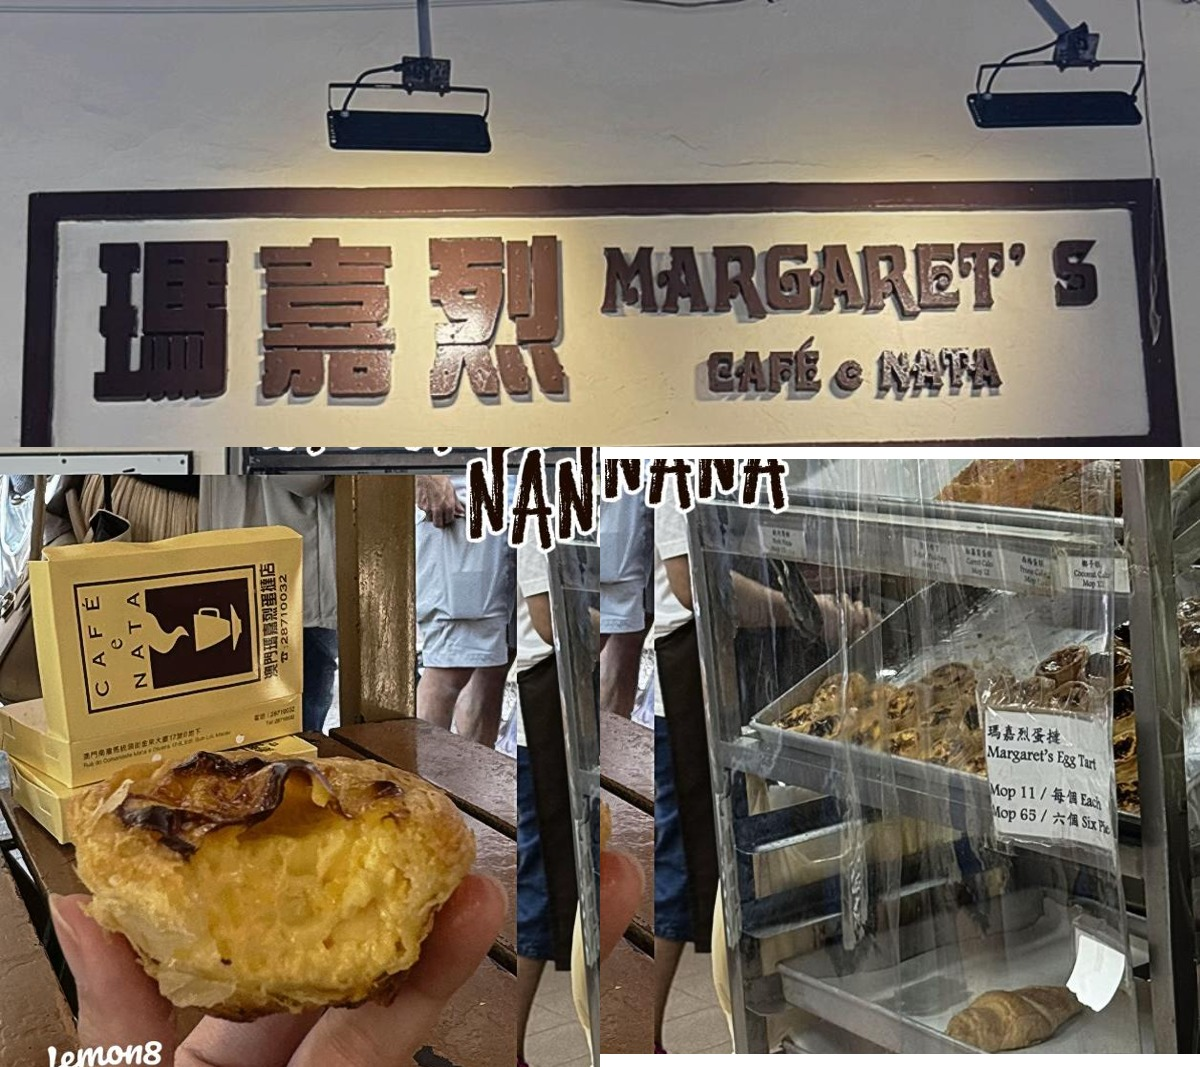
\includegraphics[width=\textwidth]{margarets_cafe_e_nata.jpg}
\end{center}
\end{column}
\begin{column}{0.52\textwidth}
\begin{itemize}
  \item \textbf{Margaret's Caf\'e e Nata} (瑪嘉烈蛋撻店)
  \item Tucked away in an alleyway near Sintra Square, it consistently generates a winding queue for its Portuguese egg tarts.
  \item Many visitors feel the tarts are overly sweet or oily compared to Lord Stow's or lesser-known local bakeries, attributing the line primarily to guidebook fame.
\end{itemize}
\end{column}
\end{columns}
\end{frame}

%--------------------------------------------------
\begin{frame}{Where else do we see herding?}
\begin{itemize}
  \item \textbf{Recent NVDA crush.} Nvidia rose with AI enthusiasm; when sentiment flipped, many investors sold together and the price fell sharply.
  \item \textbf{Bank run.} You hear a rumor the bank is in trouble; you see a long withdrawal line and join it---even if you doubt the rumor. Each extra withdrawal makes the next person more likely to run.
  \item \textbf{Homework copying.} The best econ student finishes first; the second-best compares answers with the best; the third---even if their own answer was originally correct---may switch to match the first two.
  \item Shared idea: people copy others, and that copying can push outcomes too far.
\end{itemize}
\end{frame}

%--------------------------------------------------
\begin{frame}{What is herding? (simple words)}
\begin{itemize}
  \item You have a private clue, but you also see what others chose---and sometimes you follow the crowd even when your own clue says something else.
  \item Other people's choices carry information.
  \item When signals are imprecise, early information can be wrong---so the early action can be wrong.
  \item Later arrivals infer previous players' information from their \textit{actions}, and can inherit that wrong information.
\end{itemize}
\end{frame}

%--------------------------------------------------
\begin{frame}{Setup}
\begin{itemize}
  \item \textbf{State}: one restaurant is $G$ or $B$, with prior $\Pr(G)=\Pr(B)=\tfrac12$.
  \item \textbf{Signal}: people arrive one by one; each gets $g$ or $b$ (70\% accurate), \textit{conditionally independent} given the state:
  \[
  \begin{aligned}
  \Pr(g\mid G)&=0.7,&
  \Pr(b\mid G)&=0.3,\\
  \Pr(g\mid B)&=0.3,&
  \Pr(b\mid B)&=0.7.
  \end{aligned}
  \]
  \item \textbf{Action}: \textbf{Line up} or \textbf{Drop}.
  \item \textbf{Break-even}: Line up if $\Pr(G\mid \text{info}) > \tfrac12$; Drop if $< \tfrac12$; if $= \tfrac12$, choose each with probability $\tfrac12$.
  \item Goal: Person 1--3; show Person 3 \textit{discards} his own signal.
\end{itemize}
\end{frame}

%--------------------------------------------------
\begin{frame}{Person 1 --- Bayes' rule}
\begin{center}
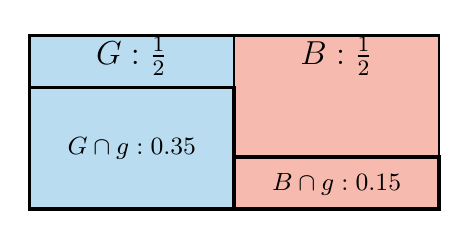
\begin{tikzpicture}[x=5.2cm,y=2.2cm]
  \fill[lightblue] (0,0) rectangle (0.5,1);
  \fill[lightcoral] (0.5,0) rectangle (1,1);
  \draw[thick] (0,0) rectangle (1,1);
  \draw[thick] (0.5,0) -- (0.5,1);
  \draw[line width=1.3pt] (0,0) rectangle (0.5,0.7);
  \draw[line width=1.3pt] (0.5,0) rectangle (1,0.3);
  \node at (0.25,0.88) {\large $G:\tfrac12$};
  \node at (0.75,0.88) {\large $B:\tfrac12$};
  \node at (0.25,0.35) {\small $G\cap g:0.35$};
  \node at (0.75,0.14) {\small $B\cap g:0.15$};
\end{tikzpicture}
\end{center}
\vspace{0.1em}
\begin{align*}
\Pr(G\mid g)
&=
\frac{\Pr(G\cap g)}{\Pr(g)}
=
\frac{\Pr(G\cap g)}{\Pr(G\cap g)+\Pr(B\cap g)}
=
\frac{\Pr(g\mid G)\,\Pr(G)}{\Pr(g\mid G)\,\Pr(G)+\Pr(g\mid B)\,\Pr(B)}\\[0.25em]
&=
\frac{0.7\cdot\tfrac12}{0.7\cdot\tfrac12+0.3\cdot\tfrac12}
=
0.7
> \tfrac12
\quad\Rightarrow\quad
\textbf{Line up.}
\end{align*}
\end{frame}

%--------------------------------------------------
\begin{frame}{Person 2}
\begin{itemize}
  \item Sees Person 1 \textbf{Line up} $\Rightarrow$ $s_1=g$.
  \item Case $s_2=g$: two good clues $\Rightarrow$ posterior $> \tfrac12$ $\Rightarrow$ \textbf{Line up}.
  \item Case $s_2=b$:
  \[
  \Pr(G\mid s_1=g,s_2=b)
  =
  \frac{\Pr(s_1=g,s_2=b\mid G)\,\Pr(G)}{\Pr(s_1=g,s_2=b\mid G)\,\Pr(G)+\Pr(s_1=g,s_2=b\mid B)\,\Pr(B)}
  \]
  \[
  =
  \frac{0.21\cdot\tfrac12}{0.21\cdot\tfrac12+0.21\cdot\tfrac12}
  =
  \tfrac12.
  \]
  Indifferent: \textbf{Line up} or \textbf{Drop} with probability $\tfrac12$ each.
\end{itemize}
\end{frame}

%--------------------------------------------------
\begin{frame}{Person 3 --- write the posterior}
\begin{itemize}
  \item Sees two people \textbf{Line up} ahead; own signal is $b$.
  \item Whether to wait (Line up) or leave (Drop) depends on
  \[
  \Pr(G\mid \mathrm{LU},\mathrm{LU},b)
  =
  \frac{\Pr(\mathrm{LU},\mathrm{LU},b\mid G)\,\Pr(G)}{\Pr(\mathrm{LU},\mathrm{LU},b\mid G)\,\Pr(G)+\Pr(\mathrm{LU},\mathrm{LU},b\mid B)\,\Pr(B)}.
  \]
  \item Need the conditional probabilities $\Pr(\mathrm{LU},\mathrm{LU},b\mid G)$ and $\Pr(\mathrm{LU},\mathrm{LU},b\mid B)$.
\end{itemize}
\end{frame}

%--------------------------------------------------
\begin{frame}{Person 3 --- conditional probabilities under $G$ and $B$}
\begin{itemize}
  \item Conditionally independent given the state:
  \[
  \Pr(\mathrm{LU},\mathrm{LU},b\mid \text{state})
  =
  \Pr(\mathrm{LU},\mathrm{LU}\mid \text{state})\,\Pr(b\mid \text{state}).
  \]
  \item Under $G$:
  \[
  \Pr(\mathrm{LU},\mathrm{LU},b\mid G)
  =
  \bigl[0.7\bigl(0.7+0.3\cdot\tfrac12\bigr)\bigr]\cdot 0.3
  =
  0.1785.
  \]
  \item Under $B$:
  \[
  \Pr(\mathrm{LU},\mathrm{LU},b\mid B)
  =
  \bigl[0.3\bigl(0.3+0.7\cdot\tfrac12\bigr)\bigr]\cdot 0.7
  =
  0.1365.
  \]
\end{itemize}
\end{frame}

%--------------------------------------------------
\begin{frame}{Person 3 --- combine and decide}
\begin{itemize}
  \item With $\Pr(G)=\Pr(B)=\tfrac12$:
  \[
  \Pr(G\mid \mathrm{LU},\mathrm{LU},b)
  =
  \frac{0.1785\cdot\tfrac12}{0.1785\cdot\tfrac12+0.1365\cdot\tfrac12}
  \approx 0.57 > \tfrac12.
  \]
  \item Compare: if he only saw the two Line-ups,
  \[
  \Pr(G\mid \mathrm{LU},\mathrm{LU})
  =
  \frac{0.595}{0.595+0.195}
  \approx 0.75;
  \]
  if he only had his private signal, $\Pr(G\mid b)=0.3$.
  \item So Person 3 still \textbf{Line up}---he discards his own signal $b$: the information from previous players' actions outweighs his private signal. Cascade starts.
\end{itemize}
\end{frame}

%--------------------------------------------------
\begin{frame}{Takeaways}
\begin{itemize}
  \item If everyone used only their own signal and we aggregated, private information would keep entering the public record.
  \item In a cascade, choices are sequential: early actions become public clues, so later people may rationally ignore their own signals.
  \item Same logic: Margaret's queues, NVDA, bank runs.
\end{itemize}
\vspace{0.4em}
\begin{center}
\large Questions?
\end{center}
\end{frame}

\end{document}
